\documentclass[12pt,twoside]{article}

\usepackage{amsthm}
\usepackage{amsmath}
\usepackage{amssymb}
\usepackage{amsfonts}
\usepackage[margin=1in]{geometry}
\usepackage{enumerate}

\usepackage{graphicx}
\usepackage{hyperref}

\newtheorem{thm}{Theorem}
\newtheorem{lemma}[thm]{Lemma}

\newcommand{\mbf}{\mathbf}
\newcommand{\mrm}{\mathrm}

\newenvironment{centered}[0]{%
  \begin{list}{}{%
    \setlength{\topsep}{0pt}%
    \setlength{\leftmargin}{.25in}%
    \setlength{\rightmargin}{.25in}%
    \setlength{\listparindent}{\parindent}%
    \setlength{\itemindent}{\parindent}%
    \setlength{\parsep}{\parskip}%
  }
  \item[]}{\end{list}}

\setcounter{tocdepth}{1}


\title{A Survey of Spectral Sparsification \\
        6.854 Final Project}
\date{\today}
\author{Robi Bhattacharjee\thanks{Massachusetts Institute of Technology - robibhat@mit.edu} \\
        Victor Pontis\thanks{Massachusetts Institute of Technology - vpontis@mit.edu} } 

\begin{document}

\maketitle

\abstract{
A spectral sparsification algorithm takes an input graph and returns a new graph with fewer edges that preserves, up to an approximation, a term called the Laplacian of the graph. The Laplacian of the graph relates to the connectivity of the graph and is a strong property: graphs with similar Laplacians also have similar cut values, similar connectivities, and other important properties. 
  
In this paper we give an introduction to spectral graph theory and sparsification. We describe two sampling algorithms: one that considers vertex degree and the other effective resistance, giving intuition behind both algorithms. We also provide the necessary background knowledge, including material in linear algebra and effective resistance, needed for analysis of the algorithms presented. We finish by commenting on the inherently linear algebraic properties of spectral sparsification and the difficulty of finding a purely combinatorial analysis.
}

\tableofcontents

\section{Background}

\subsection{Spectral Sparsification}

In a sparse graph the number of edges is on the order of the number of vertices (up to a logarithmic factor). A sparsification algorithm takes an input graph and returns a sparse graph that is an approximation of the input graph. The output sparse graph has $\tilde{O}(n)$ edges when a complete graph can have up to $O(n^2)$ edges.\footnote{For this paper we are only considering sparsification algorithms that return graphs with $\tilde{O}(n)$ edges. In general, a sparsification algorithm can return a graph with more edges but with the key property that it has less edges than the input graph. We are also only considering connected graphs. If given a graph that is not connected we can split it into connected components.} Benczur and Karger introduced the notion of sparsifiers in  \cite{benczur-karger-mincut} with the definition of cut sparsifiers. They defined a class of sparsification algorithms called cut sparsifiers which return a cut approximation, a sparse graph that approximately preserves the cut between any two sets of vertices. They used their sparsification algorithm to improve runtimes on min-cut and max-flow. 

In this paper we will be studying spectral sparsification algorithms which return spectral approximations.\footnote{We also restrict our study to sparsification algorithms where the edges in $\tilde{G}$ are a subset of the edges in $G$. So our sparsification algorithms simply reweigh edges of $G$.} Spectral approximation can be thought of as a generalization of cut approximation that preserves a term called the Laplacian, $L_G$, of a graph $G$ as defined here
%
\begin{equation}
\label{eqn:laplacian-matrix-def}
L_G(u,v) = 
            \begin{cases} 
                -w_{(u,v)}           &\mbox{if } u \not= v \\
                \sum_z w_{(u,z)}     &\mbox{if } u = v. 
            \end{cases}
\end{equation}
%
We can also write the Laplacian in its quadratic form
%
\begin{equation}
\label{eqn:laplacian-vertex-def}
x^T L_G x = \sum w_{(u,v)} (x_u-x_v)^2.
\end{equation}

From this quadratic form of the Laplacian we see the that spectral sparsification is a generalization of cut sparsification. Consider any set $S \subset V$ and let $x_S$ be the vector defined as $x(u) = 1$ if $u \in S$, and $x(u) = 0$ otherwise. Then it is clear that $x_S^T L_G x$ is just equal to the sum of the weights of the edges that span $S$ to $V - S$.\footnote{In the future we will refer to the edges that cross the cut between $V$ and $V-S$ as $E(S, V-S)$.} This shows that spectral sparsifiers are at least as strong as cut sparsifiers (they are in fact strictly stronger, but this requires more analysis). 
 
For the formal definition of spectral approximation, we let $\tilde{G}$ be a graph with the same vertices as $G$. $\tilde{G}$ is said to be a \emph{$(1+\epsilon)$-spectral approximation} if for all $x$
%
\begin{equation}
\label{eqn:spectral-sparsifier-def}
(1-\epsilon) x^T L_G x \leq x^T L_{\tilde{G}} x \leq (1+\epsilon) x^T L_G x.
\end{equation}

\subsection{Linear Algebra Background} 

In this section, we go over some linear algebra that will be useful for the analysis of graphs and sparsification algorithms.

The spectral theorem for Hermitian operators in linear algebra states that for any symmetric matrix, all of its eigenvalues are real and that its eigenvectors can be chosen to form an orthonormal basis of its domain. This theorem is central to our analysis of spectral sparsification.

In addition to the spectral theorem, we also use a list of basic linear algebra facts and notation listed below.

\begin{enumerate}
    \item If a symmetric matrix has orthonormal eigenvectors $x_1, x_2, ... , x_n$ with eigenvalues $0 = \lambda_1 < \lambda_2 < \cdots  < \lambda_n$ then for all $x \neq 0$, $\lambda_1 \leq \frac{x^TAx}{x^Tx} \leq \lambda_n$.
    \item For a given matrix $M$ we use $\lambda_i(M)$ to denote the $i$th smallest magnitude eigenvalue. This definition will only be applied to matrices with real eigenvalues.
    \item The 2-norm of a symmetric matrix $||A||$ is equal to the absolute value of its largest eigenvalue.
\end{enumerate}


\subsection{Graph Conductance}

The conductance of a graph measures the connectivity of the graph.\footnote{Our definition of conductance only applies to unweighted graphs.} The conductance of a cut considers the number of edges on both sides of the cut and the number of crossing edges. A graph cut will have low conductance if there are a lot of edges on either side but few crossing edges. We define the volume of a set $S$ of vertices such that $\text{Vol}(S)=\sum_{i\in S} d_i$  where $d_v$ denotes the degree of vertex $v$. Now we can define the conductance of a cut dividing a graph into two disjoint sets $S$ and $V-S$:
%
\begin{equation}
\label{eqn:conductance-def}
\Phi_G(S) = \frac{|E(S,V-S)|}{\text{min}(\text{Vol}(S),\text{Vol}(V-S))}.
\end{equation}
%
The conductance of the graph $G$ takes the minimum $\Phi_G(S)$ over all $S$ so that 
%
\begin{equation}
\Phi_G = \underset{\emptyset \not= S \subset V}{\text{min}} \Phi_G(S).
\end{equation}

A graph with high conductance has high connectivity and it is hard to partition off a set of vertices from the rest of the graph. On the other hand, a graph with low conductance has low connectivity and we are able to partition the graph into disjoint sets where the boundary between the sets is small. 

Conductance is also closely related to the Laplacian of a graph as we show in Cheeger's Inequality below. Before describing this, we first define the normalized Laplacian. The normalized Laplacian is the matrix
%
\begin{equation}
\label{def:normalized-laplacian}
\mathcal{L}_G = D^{-1/2}L_GD^{-1/2}
\end{equation}
%
where $D$ is the diagonal matrix defined by $D(u,v) = 0$ if $u \neq v$ and $D(v,v) = d_v$. The normalized Laplacian of a graph satisfies a similar equation to (\ref{eqn:laplacian-vertex-def}):

\begin{equation}
\label{eqn:norm-laplac}
x^T \mathcal{L}_G x = \sum_{(u,v) \in E} \left(\frac{x_u}{\sqrt{d_u}}-\frac{x_v}{\sqrt{d_v}}\right)^2.
\end{equation}

\section{Sampling by Vertex Degree}

\subsection{Cheeger's Inequality} % and intutition
Cheeger's Inequality connects the conductance $\Phi_G$ with $\lambda_2(\mathcal{L})$. This allows us to analyze the eigenvalues of the normalized Laplacian in place of conductance. It states that

\begin{thm}
$2\Phi_G \geq \lambda_2(\mathcal{L}) \geq \Phi_G^2/2$.
\end{thm}

\begin{proof}
We first prove that $\lambda_2(\mathcal{L}) \geq \Phi_G^2/2$. The full proof of this is quite involved, so we'll only give a sketch.
    The basic idea is to start with the eigenvector $x$ such that $\mathcal{L}x = \lambda_2x$. Then, sort the vertices $v$ based on the magnitude of $x(v)$ to get $x(v_1) \leq x(v_2) \leq \cdots \leq x(v_n)$. The idea then becomes to show that we can find $i$ such that $\lambda_2 \geq \Phi_{S_i}^2/2$ where $S_i = \{v_1, v_2, \cdots, v_i\}$. The intuition behind this is somewhat analogous to the proof of the other direction in the inequality. Consider any set $S_i$. Intuitively, edges that span from $S_i$ to $V-S_i$ are expected to have a larger value of $(\frac{x_v}{\sqrt{d_v}} - \frac{x_u}{\sqrt{d_u}})^2$ than edges that stay contained within $S_i$ or $V-S_i$. So the idea of the proof is that if there are many edges from $S_i$ to $V-S_i$, then the Laplacian will be large. Of course, this isn't necessarily true for any one value of $S_i$, but over the group of them, it can be shown that this idea works. Interested readers can see \cite{cheeger} for the full proof.

For the other side of the inequality, we'll provide a more full proof. The main intuition behind the proof is that if you have a set $S$ such that $\Phi_G(S)$ is very small, then you can create a vector $x$ for which $\frac{x^T\mathcal{L}x}{x^x}$ is also small. This is done by making the values of $x(v)$ where $v \in S$ large and positive, and the values of $x(v)$ where $v \in V-S$ negative. We now formalize this intuition.

First, consider the set $S$ such that $\Phi_G(S) = \Phi_G$ and such that $\text{Vol}(S) \leq \text{Vol}(V-S)$. Let $e,f > 0$ be positive real numbers that will be specified later. Then let $x$ denote the vector defined by
%
\begin{equation*}
x(v)  = 
            \begin{cases}
                e\sqrt{d_v}     &\mbox{if $v \in S$} \\
                -f\sqrt{d_v}    &\mbox{if $v \notin S$}. \\
            \end{cases}
\end{equation*}
%
Then it follows from (\ref{eqn:norm-laplac}) that
%
\begin{equation*}
\frac{x^T\mathcal{L}x}{x^Tx} = \frac{(e+f)^2|E(S,V-S)|}{e^2\text{Vol}(S) + f^2\text{Vol}(V - S)}.
\end{equation*}

We now select $e,f$ such that $\sum_{v \in S} e d_v = \sum_{v \in V-S} f d_v$. This implies that $x$ is orthogonal to the vector $y$ defined by $y(v) = \sqrt{d_v}$. Therefore, we must have that $\lambda_2(\mathcal{L}) \leq \frac{x^T \mathcal{L} x}{x^T x} $ since $y$ can easily be verified to be the vector with eigenvalue 0 with respect to $\mathcal{L}$.\footnote{We use the variational theorem to state that $\frac{x^T M x}{x^Tx}$ is greater than the first positive eigenvalue if $x$ is orthogonal to the smallest eigenvector of $M$ and all of the eigenvalues are real and greater or equal to zero.} However, we have that
%
\begin{equation}
\lambda_2(\mathcal{L}) \leq \frac{x^T\mathcal{L}x}{x^Tx}  
    = \frac{(e+f)^2|E(S,V-S)|}{(e + f)e\text{Vol}(S)}
    = \frac{(e+f)\Phi_G}{e} \leq 2\Phi_G
\end{equation}
%
by substituting that $e\text{Vol}(S) = f\text{Vol}(V-S)$ and by using the fact that since $\text{Vol}(S) \leq \text{Vol}(V - S)$, $e \geq f$. This gives us what we wanted and we are done.
 

\end{proof}


\subsection{Algorithm}

In this section we present an algorithm for generating a $(1+\epsilon)$-spectral approximation of an unweighted graph by sampling with probability proportional to vertex degree. Instead of providing the entire algorithm, we focus on the portion that we feel is most relevant. We define a sub-routine \textbf{Sample} which creates a spectral sparsifier of $G$ only if $G$ has high conductivity (and consequently a high second eigenvalue by Cheeger's Inequality). The full algorithm works by partitioning the the input graph into sections of high conductivity and then applying the sampling routine. The rest of this section just concerns the sampling routine.

We define $\text{\textbf{Sample}}(G, \epsilon, \lambda)$ where $G$ is a graph with $\lambda_2(L_G) \geq \lambda$, and $\epsilon$ is a real number between 0 and 1/2 to be the following routine: select each edge $e$ with probability $p_e$ and add selected edges to the output graph with weight $1/p_e$. 

\begin{thm}[Sampling by degree]
\label{thm:sample-by-degree}
Suppose we run $\normalfont{\textbf{Sample}}(G, \epsilon, \lambda)$ such that
%
\begin{equation*}
\forall (u,v) \in E.\:\, p_e = \text{min}(1, C/\text{min}(d_u, d_v)) \text{ where } C=\Theta((\log n)^2 (\epsilon\lambda)^{-2})
\end{equation*}
%
and get an output graph $\tilde{G}$.  With probability of at least $1/2$ $\tilde{G}$ is a $(1+\epsilon)$-spectral approximation of $G$ with an average degree of $O((\log n)^2 (\epsilon \lambda)^{-2})$. 
\end{thm}

This theorem from \cite{microsoft-summary} shows that the number of edges that we need to sample to get a spectral approximation will depend on the connectivity of the graph due to the $\lambda^{-2}$ term included in $p_e$ with low connectivity graphs needing more edges. 

%We see from Cheeger's inequality that $\lambda_2$ is large when we have large conductance and thus high connectivity, so our algorithm works best on graphs that have high connectivity. In the paper \cite{spielman-teng-spectralsparse}, the input graph is partitioned into subgraphs that have high connectivity and this algorithm is run as a subroutine on these subgraphs.

\subsection{Analysis}

At a very high level, the basic idea of the proof of Theorem \ref{thm:sample-by-degree} is to prove that 

\begin{enumerate}
    \item $\tilde{G}$ is NOT a $(1 + \epsilon)$ approximation of $G$ with probability at most $1/3$.
    \item $\tilde{G}$ has more than $O\left(\frac{(\log n)^2}{\epsilon^2\lambda^2}\right)$ edges with probability at most $1/6$.
\end{enumerate}

Since $P(A \cup B) \leq P(A) + P(B)$, the probability that $\tilde{G}$ doesn't satisfy the desired properties would be at most 1/2 meaning that it works with probability at least 1/2. We now show how to obtain the two claims above. 

\begin{lemma}
\label{lem:spectral-approximation}
Let $\tilde{L}$ denote the Laplacian of $\tilde{G}$. Then if $||D^{-1/2}(L-\tilde{L})D^{-1/2}|| \leq \delta$, $\tilde{G}$ is a $(1+\epsilon)$-spectral-approximation of $G$ where $\epsilon = \frac{\delta}{\lambda_2}$.\footnote{$D$ is the same diagonal matrix we used in (\ref{def:normalized-laplacian})}
\end{lemma}

\begin{proof}
This lemma is quite simple to prove with some basic linear algebra. The basic idea is that 
%
\begin{equation*}
D^{-1/2}\tilde{L}D^{-1/2} = D^{-1/2}LD^{-1/2} + D^{-1/2}(\tilde{L} - L)D^{-1/2}
\end{equation*}
%
means that if $D^{-1/2}LD^{-1/2}$ is large and $D^{-1/2}(\tilde{L} - L)D^{-1/2}$ is small, the ratio between $D^{-1/2}LD^{-1/2}$ and $D^{-1/2}\tilde{L}D^{-1/2}$ will be close to 1. Since eigenvalues naturally relate to the Laplacian form and to the "size" of a matrix, the rest of the work is just formalizing this idea in terms of algebra. Interested readers can find a full proof in \cite{spielman-teng-spectralsparse}.

\end{proof}

This lemma conveys an important idea that dictates the rest of our proof. It basically means that given a sufficiently well connected graph (i.e. a graph of high conductance), it suffices to bound the 2-norm of the difference between normalized Laplacians. Therefore, in order to prove the original theorem, since we already know that $\lambda_2(\mathcal{L}) \geq \lambda$, it suffices to analyze the distribution of $||D^{-1/2}(\tilde{L} - L)D^{-1/2}||$. 

To do this, we notice that 
%
\begin{equation}
||D^{-1/2}(\tilde{L} - L)D^{-1/2}|| \leq ||D^{-1/2}(\tilde{A} - A)D^{-1/2}|| + ||D^{-1/2}(\tilde{D} - D)D^{-1/2}||
\end{equation}
%
from $A + L = D$ where $A$ denotes the adjacency matrix and $D$ denotes the diagonal matrix of vertex degrees. We analyze each of those terms separately. It turns out that they both are easier to analyze than analyzing the Laplacian directly.

Finding the distribution of $||D^{-1/2}(\tilde{D} - D)D^{-1/2}||$ is relatively easy. This is because the eigenvalues of a diagonal matrix are just the diagonal entries themselves. Consequently, bounding the maximum eigenvalue can be done by using a union bound and a Chernoff bound. The union bound comes from the fact that in order for the maximum diagonal entry to be large, one of the diagonal entries needs to be large so we have to bound the probability of this happening. The Chernoff bound comes from the fact that the diagonal entries of $\tilde{D}$ are just sums of random variables. Together, it can be shown that

\begin{equation}
\text{Pr}[||D^{-1/2}(D - \tilde{D})D^{-1/2}|| \geq \epsilon\lambda/3] \leq 1/6.
\end{equation}

The distribution of $||D^{-1/2}(\tilde{A} - A)D^{-1/2}||$ is a little more tricky to analyze. First of all, for any matrix $B$, conjugating by an invertible matrix $C$ to get $CBC^{-1}$ preserves the eigenvalues of $B$. Consequently, it is equivalent to analyze the distribution of $||\Delta|| = ||D^{-1}(\tilde{A} - A)||$.  

There are two main ideas in analyzing the eigenvalues of $\Delta$. First of all, we can bound the largest eigenvalue by bounding the trace of $\Delta^m$ for some even number $m$. This is because the trace of a matrix is equal to the sum of its eigenvalues. (The point of $m$ being even is to get rid of cases with negative eigenvalues.) The second key idea is to relate the entries in the matrix $\Delta^m$ to taking random walks in $G$. 

The rest of the proof basically analyzes an arbitrary entry of $\Delta^m$. From the definition of matrix multiplication, $\Delta^m(u,v)$ basically is the sum over all paths of length $m$ from $u$ to $v$ of the product of the edges on the path. This product is then bounded by noticing that in expectation, any path that uses an edge only once has expected value 0 since each edge has expected weight 0 as $E(\tilde{A}) = A$ because the expected of each edge in $\title{G}$ is equal to its weight in $G$. Therefore, by looking at paths that use edges at least twice and pairing entries $\Delta(a,b)$ with $\Delta(b,a)$, one can obtain a bound the eventually leads to


\begin{equation}
\text{Pr}[||D^{-1/2}(\tilde{A} - A)D^{-1/2}|| \geq \epsilon\lambda/3] \leq 1/6.
\end{equation}

Therefore, combining these we see that $\tilde{G}$ is NOT a $(1 + \epsilon)$ approximation of $G$ with probability at most $1/3$. To get the other part of the theorem, we can easily use a Chernoff bound to get a bound on the number of edges appearing in the graph. This gives us that $\tilde{G}$ has more than $O\left(\frac{(\log n)^2}{\epsilon^2\lambda^2}\right)$ edges with probability at most $1/6$. This finishes up the proof.


\section{Sampling by Effective Resistance}

% effective resistance overview 
\subsection{Effective Resistance Background}

The effective resistance in graphs derived from electrical networks shows great promise as a new, powerful measure of distance and gives important contributions to the analysis of spectral graph theory. In the overview, we will define effective resistance by modeling the graph as an electrical network, connect effective resistance to the Laplacian, and look at the relationship between commute time and effective resistance. Then we examine an algorithm that samples edges with probabilities proportional to their effective resistance and give an analysis. 

\subsubsection{Calculating Effective Resistance}

% laws of effective resistance 

In order to understand effective resistance, we need to remember two laws from electromagnetism, Ohm's and Kirchoff's. Ohm's Law states that $V=ir$ if $V$ is voltage, $i$ current, and $r$ resistance. Kirchoff's Law requires the conservation of current, stating the current into any vertex is equal to the current leaving the vertex. The effective resistance between two vertices $u$ and $v$ is then equal to the voltage differential between the two when a unit of current is injected into $u$ and a unit of current is extracted from $v$.

% calculating effective resistance 

Calculating the effective resistance on a small circuit is easy. When we have resistors in series we simply add them and when we have resistors in parallel we combine their inverses. We can then iteratively apply these two methods to combine all of the resistors into one, yielding the effective resistance between two vertices. This gets much more complicated as the circuit gets larger and below we give an expression of effective resistance in terms of eigenvalues of the Laplacian. 


\subsubsection{Connection to Laplacian}

In this section we will relate effective resistance to the Laplacian through a series of matrix operations. We begin by defining a matrix $B$. We arbitrarily order the edges on our graph and define $B$ as an $m \times n$ matrix where

\begin{equation}
\label{def:resistance-b}
B(e,v)  = 
            \begin{cases}
                1     &\mbox{if $v$ is $e$'s head} \\
                -1    &\mbox{if $v$ is $e$'s tail} \\
                0     &\mbox{otherwise.} 
            \end{cases}
\end{equation}

In our definition of effective resistance, we injected a current of $1$ into a vertex $v$ and injected a current of $-1$ into a vertex $u$. The natural generalization of this identity is to have an $n$-dimensional vector $i_{\text{ext}}$ where $i_{ext}(v)$ denotes the amount of current injected into vertex $v$. We also set $i$ to be the $m$-dimensional vector such that $i(e)$ denotes the amount of current flowing across edge $e$.\footnote{We define a positive value of $i(e)$ to represent current flowing across $e$ in the same direction that $B$ orients $e$.} From these simple definitions, we get the equation $B^Ti = i_{\text{ext}}$. This equation can be verified as an expression of Kirchoff's Law.

It is also quite natural to consider the n-dimensional vector $v$ as the potential at each vertex. The potential differential by any two vertices is uniquely determined by the current and resistance on the edges of the graph. Let $W$ be the $m \times m$ diagonal matrix so that $W(e,e) = w_e$. Then by Ohm's law, we have that $i = WBv$. 

Combining both of these equations we can get that $i_{\text{ext}} = B^TWBv$. We also notice through matrix multiplication that $B^TWB$ is equal to the Laplacian. This means that
%
\begin{equation*}
i_{\text{ext}} = B^TWBv = Lv.
\end{equation*}

The connection of this equation to effective resistance is quite clear. To compute the effective resistance of the edge $(u,v)$, we set $i_{\text{ext}}$ to the vector corresponding to injecting one unit of current into $u$ and taking out one unit of current from $v$. Then, we solve the above equation to get $v$ and thereby obtain the potential difference which is equal to effective resistance. Consequently, it is quite natural to try to consider some sort of inverse of $L$. 

The Laplacian has one eigenvalue of zero\footnote{In following with the assumptions in the rest of the paper, we assume that the graph is connected. In a graph that is not connected we will have multiple eigenvalues of zero.} so we are not able to take normal inverse of the Laplacian\footnote{When we have an eigenvalue of zero that means the determinant is zero and the matrix is non-invertible.}. Instead we define the \textit{Moore-Penrose Pseudoinverse}, $L^+$, such that $LL^+ = L^+L$ projects into the column space of the Laplacian. Now we recall the spectral theorem and decompose each matrix into a sum of eigenvectors, giving the following definitions
%
\begin{eqnarray}
L = \sum\limits_{i=2}^{n} \lambda_i u_i u_i^T & L^+ = \sum\limits_{i=2}^{n} \dfrac{1}{\lambda_i} u_i u_i^T & L^+L = \sum\limits_{i=2}^{n} u_i u_i^T
\end{eqnarray}
%
where the $\lambda_i$'s are eigenvalues and the $u_i$'s are their corresponding orthonormal eigenvectors. Now we get the effective resistance $R_{uv}$ between vertices $u$ and $v$ to be 

\begin{eqnarray}
R_{uv} &=& (\mbf{e}_u - \mbf{e}_v)^T L^+ (\mbf{e}_u - \mbf{e}_v) \\
       &=&  L^+_{uu} -2L^+_{uv} + L^+_{vv}. 
\end{eqnarray}

Here we can see that the effective resistance is inextricably tied to the Laplacian.

\subsubsection{Connection to Commute Time}

In this section, we relate the effective resistance to a property of random walks called commute time. A random walk on a graph begins at a vertex and at each step follows an edge incident on the current vertex with uniform probability. The hit time between $u$ and $v$ is the expected time a random walk will take to traverse from $u$ to $v$. The commute time from $u$ to $v$ is expected time to get from $u$ to $v$ and back to $u$ again, or the sum of the hit times from $u$ to $v$ and from $v$ to $u$. The commute time will be small if there are a lot of short paths between vertices. 

We are able to relate commute time to effective resistance with the following lemma
%
\begin{lemma}
\label{lem:commute-time-effective-resist}
If we look at two vertices $u$ and $v$ and call the commute time $C_{uv}$ and the effective resistance $R_{uv}$ we can get a relation between the two in the form $C_{uv} = 2m R_{uv}$.
\end{lemma}
%
We will not prove this lemma but it it is proven in \cite{wisc-effective-resistance} and gives us a nice connection between commute time and effective resistance.

\subsection{Algorithm}

Spielman and Srivastava introduced an alternative sampling algorithm for generating a spectral sparsifier of $O(n\log n/\epsilon^2)$ edges in nearly linear time based on effective resistance. Their paper \cite{spielman-effective-resistance} defines a sparsify algorithm that runs as follows

\begin{centered}
$H$ = \textbf{Sparsify}$(G,q)$

Choose a random edge $e$ with probability $p_e$ proportional to $w_e R_e$ and add $e$ to $H$ with weight $w_e/qp_e$. Take $q$ samples independently with replacement, summing weights if an edge is chosen more than once. 
%\rule{10}{10}
\end{centered}

This algorithm picks exactly $q$ edges total. Each edge it picks is randomly selected. This means that $\sum_e p_e = 1$. The paper also proves the following theorem

\begin{thm}
Suppose we have $G$ and $H$ = \normalfont{\textbf{Sparsify}}$(G, q)$ and $1/\sqrt{n} < \epsilon \leq 1$. If $q=O(n\log n /\epsilon^2)$ and $n$ is sufficiently large than with probability at least half $H$ is a $(1+e)$-spectral approximation of $G$.
\end{thm}

It makes sense to sample with probability related to effective resistance because we know that an edge connecting $u$ and $v$ has effective resistance 1 then it is the only path from $u$ to $v$, any other path would lower the effective resistance. So this edge must be picked. Effective resistance is a strong signal for the importance of an edge. 

\subsection{Analysis}

We seek to show that for all $x$, 
%
\begin{equation*}
\frac{|x^T\tilde{L}x - x^TLx|}{x^TLx} \leq \epsilon.
\end{equation*}
%
The idea behind doing this is to slightly strengthen the claim so as to eliminate the need for the messy term $x$. More concretely, let $S$ be the diagonal matrix such that 
%
\begin{equation}
S(e,e) = \frac{\tilde{w_e}}{w_e} = \frac{(\text{number of times e is sampled})}{qp_e}.
\end{equation}
%
The point of this is that 
%
\begin{equation}
L = B^TWB \rightarrow
\tilde{L} = B^T\tilde{W}B = B^TW^{1/2}SW^{1/2}B.
\end{equation}
%
Given these, we do the following manipulations:
%
\begin{equation*}
\frac{|x^T\tilde{L}x - x^TLx|}{x^TLx} = \frac{|x^TB^TW^{1/2}SW^{1/2}Bx - x^TB^TWBx|}{x^TB^TWBx} = \frac{y^T(S-I)y}{y^Ty}
\end{equation*}
%
where $y = W^{1/2}Bx$. This is nice because the expression $\frac{y^T(S-I)y}{y^Ty}$ strongly suggests analyzing the norm of the matrix $(S-I)$. Unfortunately, this doesn't quite work. $y$ does not range over all vectors as $x$ does: $y$ is always in the range of $W^{1/2}B$ which is not an invertible matrix. This means that while $||S - I|| \leq \epsilon$ implies our desired result, it isn't necessarily true. 

The key insight that makes this method work is the construction of a Projection matrix $\Pi$ with several key properties. $\Pi$ projects onto the space of all vectors $y$ such that $y = W^{1/2}Bx$ for some $x$. This means the $\Pi y = y$ for all $y = W^{1/2}Bx$. Furthermore, $\Pi$'s structure needs to be sufficiently simple so that analyzing it isn't too difficult. Before showing $\Pi$'s structure, we will first note that 
%
\begin{equation*}
\frac{|x^T\tilde{L}x - x^TLx|}{x^TLx} = \frac{y^T(S-I)y}{y^Ty} 
            = \frac{y^T\Pi(S-I)\Pi y}{y^Ty} \leq ||\Pi(S-I)\Pi||.
\end{equation*}
%
Therefore, it suffices to show that $||\Pi(S-I)\Pi|| \leq \epsilon$ for some matrix $\Pi$. It turns out that taking
%
\begin{equation}
\Pi = W^{1/2}BL^+B^TW^{1/2}
\end{equation}
%
works. This can be shown without too much difficulty to be a projection matrix that projects on to the space $\text{im}(W^{1/2}B)$. 

$\Pi$ is more than just an arbitrary projection matrix though. This will become evident from the analysis of $||\Pi(S-I)\Pi||$. The basic idea is as follows: based upon $\Pi$'s definition, it isn't too difficult to see that 

\begin{equation*}
\Pi S \Pi = \frac{1}{q}\sum_{e}(\text{number of times e is sampled})\frac{\Pi(e)}{\sqrt{p_e}}\frac{\Pi(e)^T}{\sqrt{p_e}}= \frac{1}{q}\sum_1^q y_iy_i^T
\end{equation*}
%
where each $y_i$ is a vector drawn from the distribution
%
\begin{equation*}
y = \Pi(e)/\sqrt{p_e} \text{ with probability } p_e.
\end{equation*}

The idea of this is that there are well known ways of analyzing the random variable $\frac{1}{q}\sum_1^q y_iy_i^T$ given the variable $y$. From here, the paper cites a well known law of large numbers for symmetric rank 1 matrices to bound the expected value of 

\begin{equation*}
||\frac{1}{q}\sum_1^q y_iy_i^T - E[yy^T]||.
\end{equation*}

From here, the rest of the proof is just a bit of simple algebra. The key idea here was finding the correct matrix $\Pi$ that had all the desired properties.

\section{Comparing the Algorithms}
\label{comparing-algorithms}

In this section we will compare and contrast the algorithms and through this process explore some properties of spectral approximations. 

% tension between high probability for each edge --> good approximation and low probability --> sparse graph
% tension between looking at each edge once and going through a number of samples
% choosing what edges are important
% commute time on vertex sampling graph could be used in place of linear algebra but this is already built into the effective resistance
% high conductance makes effective resistance and vertex degree similar

In both algorithms we assign a probability to different edges and sample edges based on their probabilities. In the vertex degree algorithm we look at each edge $e$ once and choose it with probability $p_e$. In the effective resistance algorithm we assign $p_e$'s but instead of sampling each edge we normalize all of them so that $\sum_e p_e = 1$ so that we can simply take $q$ samples of the edges on the entire graph. In the effective resistance algorithm we sample the graph as a whole rather than the edges one by one. 

We can also gain a lot from understanding the cases when the two algorithms are similar. For this we look at a result from \cite{hitting-commute-time} that relates the commute time $C_{uv}$ between $u$ and $v$ to the degrees of $u$ and $v$ in the form
%
\begin{equation}
\frac{1}{\text{Vol}(G)} C_{uv} \approx \frac{1}{d_u} + \frac{1}{d_v} \rightarrow R_{uv} \propto \frac{1}{d_u} + \frac{1}{d_v}.
\end{equation}
%
This tells us that the effective resistance between two vertices is proportional to the inverse of their degree. This result holds if a graph is ``reasonably large" and ``reasonably strongly connected". 

The sampling by degree algorithm splits the graph into subgraphs of high connectivity and runs the vertex degree sampling algorithm on these subgraphs. This partitioning into high connectivity subgraphs effectively makes the probability of each edge proportional to the effective resistance of the edge. In the limit of highly connected graphs, the probabilities we get from vertex degree begin to approximate the effective resistance probabilities. 

\begin{figure}[ht!]
\centering
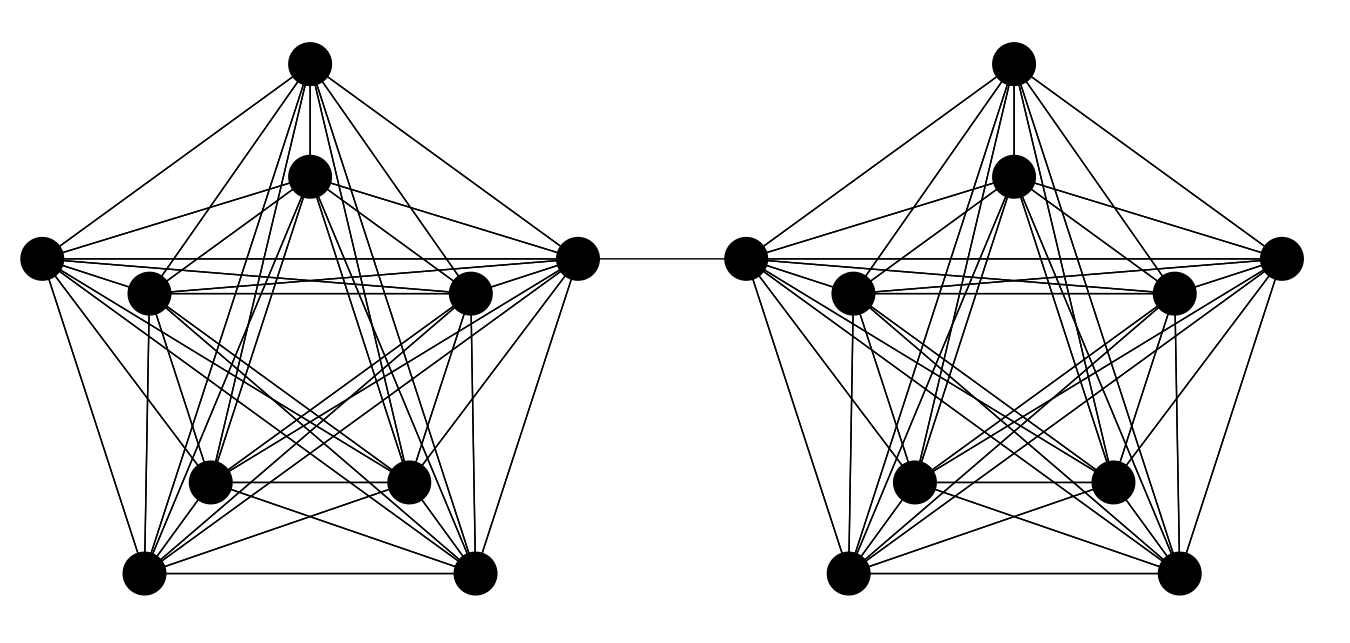
\includegraphics[width=90mm]{complete-graphs.png}
\caption{Two complete graphs joined by an edge.}
\label{complete-graphs}
\end{figure}


In graphs with low connectivity, sampling by effective resistance works while sampling by degree does not. We use an example to illustrate this. Consider two complete graphs joined by one edge $e_j$ as shown in Figure \ref{complete-graphs}.\footnote{This figure was taken from \cite{spielman-teng-spectralsparse}.} This edge is absolutely crucial to preserving the Laplacian because we can split the graph by cutting this edge. In the vertex degree sampling algorithm this edge actually is less likely to be picked than the rest of edges because the vertices on both sides of the edge have the highest degree in the graph. But the effective resistance of this edge is one, so the effective resistance sampling algorithm will always pick this edge. 

This example shows us that sampling by vertex degree must partition the graph into regions with high connectivity. Only in regions of high connectivity is the vertex degree a good indicator of the importance of an edge. This is due to the locality of the vertex degree property; it does not take into account what is happening away from that edge. Effective resistance overcomes this because it is a local property that takes the entire graph into consideration. 

\section{Linear Algebra vs Combinatorics}
One of the interesting shared features of both algorithms is that they seemingly are just random sampling algorithms. It isn't clear why linear algebra is intrinsically necessary or fundamental to this problem. In this section, we'll attempt to provide some justification and intuition supporting the necessity of linear algebra. 

Initially, we attempted find an analysis of spectral sparsification independent of linear algebra. The first step in doing this would be a definition of spectral sparsifiers that does not rely on linear algebra. 

The most natural thing to try is using the definition of a cut sparsifier. We've already shown that all cut sparisfiers are spectral sparsifiers, but the reverse does not hold. One might try to fix the definition in some way, or perhaps find a weaker-but-sufficient definition (for example, maybe a $(1 + \epsilon)$ cut sparsifier is guaranteed to be a $(1 + 2\epsilon)$ spectral sparsifier). Unfortunately, this is doomed to not work, because it turns out that verifying a cut-sparisfier is NP-hard. This means that given $G, H$, and $\epsilon$, it is NP-hard to check whether $G$ is a $(1+\epsilon)$-cut sparsifier of $H$. However, it is possible to check whether $G$ is a $(1 + \epsilon)$-spectral sparisfier of $H$ in polynomial time.

The next thing to try might be forming a definition of a spectral sparsifiers from one of the two algorithms we have for generating them. On a high level, this approach is very unlikely to work because of the natures of the proofs of correctness. Both proofs strengthened the claim first: this means that they proved that the output is not only a spectral sparsifier, but a particular kind of spectral sparisifier.

Expanding on this idea, consider the sampling by vertex-degree algorithm. Based on lemma \ref{lem:spectral-approximation},  we might try defining spectral sparsifiers based on the relationship between $||D^{-1/2}(L - \tilde{L})D^{-1/2}||$ and $\lambda_2(D^{-1/2}LD^{-1/2})$. This hypothetical definition can be made into a combinatorial interpretation by the fact that $\lambda_2(D^{-1/2}LD^{-1/2})$ is bounded by Cheeger's inequality and $||D^{-1/2}(L - \tilde{L})D^{-1/2}||$ can be bounded by the trace of a matrix which in turn is strongly related to random walks. Unfortunately, this attempt fails because graphs where $\lambda_2(D^{-1/2}LD^{-1/2})$ is 0 do indeed have spectral sparsifiers. This is why the vertex sampling algorithm is coupled with a partitioning algorithm. 

Using effective resistance seems even harder because the proof of correctness for sampling by effective resistance is heavily rooted in linear algebra. 

We conclude this section by noting another possible approach. Suppose we find a combinatorial algorithm for spectral sparsification \emph{verification}. Then, this algorithm could be used to create a combinatorial definition for spectral sparsification. Unfortunately, we weren't able to find any such algorithm, but we note that one would certainly be of interest.

\section{Conclusion}

Originally we wanted to give an overview of spectral sparsifiers and provide a combinatorial analysis of the algorithms. We found that spectral sparsification relies heavily on inherently linear algebraic properties and techniques and were not able to formulate a combinatorial analysis. Instead, we focused on the intuition behind two of the most recent sparsification algorithms. Using the shared intuition from both algorithms it is evident how sampling by effective resistance sampling improves on sampling proportional to vertex degree. Hopefully this intuition can help lead to new work in spectral sparsification. 

\bibliographystyle{alpha}
\bibliography{references}

\end{document}